\documentclass[12pt]{article}
\usepackage{amssymb}
\usepackage{graphicx}
\graphicspath{{../images/}}
\author{Andrea Malvezzi}
\title{\textbf{Logica per l'informatica~-~Lezione~1.5.\\Teorie degli insiemi (cenni)}}
\date{20 Settembre, 2024}
\begin{document}
\maketitle
\pagebreak
\section{Introduzione}
I matematici ragionano su vari elementi, alcuni concreti ed altri astratti.\\
Per fare ciò occorre assumere che questi elementi soddisfino certe proprietà, ragionando al contempo stesso sulle conseguenze di queste.
\subsection{Esempio di proposizione non sempre valida}
Un esempio significativo lo si ha con la geometria euclidea.\\
Prendendo uno dei suoi principali assiomi, ovvero "due rette parallele non si incontrano mai", si va ad esaminare una proposizione che non sempre risulta valida:
\begin{itemize}
    \item Prendendo ad esempio come concretizzazione delle due rette due segni a matita paralleli disegnati su un foglio, ovviamente i due non si incontreranno mai;
    \item Prendendo invece come concretizzazione due persone che camminano parallelarmente sulla Terra, le due potrebbero eventualmente incontrarsi, a causa della forma del pianeta.
\end{itemize}
Per rendere tale proposizione consistente occorre quindi effettuare assunzioni a loro volta consistenti, tentando di ridurre al minimo le incongruenze nel nostro pensiero.
\pagebreak
\section{Dare fondamento a un sistema logico}
Dare un fondamento a un sistema logico significa quindi, all'occorrenza, implementare un nuovo set di \textbf{enti} (concetto di cui si vuole parlare) e ipotesi partendo da un subset più piccolo che sappiamo essere consistente/coerente.\\
Partendo dal piccolo siamo quindi in grado di implementare qualcosa di nuovo.\\
Un esempio di ciò è la \textbf{teoria degli insiemi}, adottata verso il 1900 come \textbf{fondamento} per la matematica.\\
Per poter ridurre gli enti matematici a insiemi, gli enti di partenza della teoria degli insiemi devono essere il più \textit{"bassi"} ed \textit{"astratti"} possibile, escludendo quindi numeri, funzioni etc... che verranno poi implementate in seguito se necessario.
\section{La teoria degli insiemi e l'informatica}
Si può affermare che la teoria degli insiemi sia il "\textit{linguaggio macchina della matematica}".\\
Questo costituisce difatti uno strumento utile per sviluppare nuovi teoremi, implementando nuovi insiemi e fornendo così una capacità di astrazione infinita (grazie a tale fondamento si può effettivamente parlare di "infiniti numerici").\\
Inoltre un insieme è un ente molto flessibile, in quanto ogni cosa può essere considerata un insieme, ed un insieme può essere un recipiente per altri insiemi, rimanendo comunque \textbf{unitario} e non un sottoinsieme a sua volta.\\
Basti pensare a un sacchetto contenente delle biglie di 3 colori diversi: il sacchetto costituisce un insieme senza \textbf{soprainsieme}, contenente tanti altri insiemi minori (le palline di un certo colore, quelle con un certo dettaglio, etc...)\\
Tuttavia, così facendo si perde la capacità computazionale in cui l'informatica invece eccelle: basti pensare all'inefficienza nel rappresentare i dati.\\
Il numero 10, banalmente, richiede un centinaio di insiemi per essere definito e rappresentato correttamente, mentre per un calcolatore si tratta solamente di 4 bit disposti in una certa maniera.
\section{La teoria naive degli insiemi}
Fu il primo tentativo di descrivere la teoria degli insiemi da parte di Cantor.\\
Essenzialmente secondo questa teoria:
\begin{itemize}
    \item Posso formare insiemi in qualunque modo mi venga in mente.
    \begin{itemize}
        \item es. elencando gli elementi: \textit{A} = \{1, 2, 3, ...\};
        \item es. tramite \textbf{l'assioma di comprensione}: \textit{B} = \{\textit{X} | \textit{P(X)}\};  
    \end{itemize}
    \item Gli insiemi non devono essere \textbf{omogenei} (elementi anche non della stessa specie).
    \item Le ripetizioni e l'ordine non contano.
    \item I predicati sono l'uguaglianza e l'appartenenza.
\end{itemize}
Gli insiemi si possono quindi vedere (spesso) come delle scatole, ed è perciò corretto parlare di \textbf{appartenenza} e di \textbf{inclusione}.
\begin{itemize}
    \item Appartenenza ($\in$): \textit{A} è un elemento dell'insieme \textit{B} se "aprendo" \textit{B} vedo direttamente \textit{A}.
    \begin{itemize}
        \item es. di \textbf{non} appartenenza: \{1, 2\} $\notin$ \{1, 2, 3\} in quanto \{1, 2\} sono contenuti in una scatola a sé (in un sottoinsieme quindi);
        \item es. di appartenenza: 1 $\in$ \{1, 2, 3\} in quanto 1 non è contenuto in un'altra scatola.
    \end{itemize}
    \item inclusione ($\subset$): \textit{A} è sottoinsieme di \textit{B} sse aprendo le scatole vedo tutti gli elementi di \textit{A} anche in \textit{B}.
    \begin{itemize}
        \item es. di \textbf{non} inclusione: \{1, 3\} $\not \subset$ \{\{1, 2\}, 3\}, in quanto aprendo sia l'insieme \textit{A} (\{1, 2\}) che quello \textit{B} (\{\{1, 2\}, 3\}) non si vedono direttamente tutti gli elementi di \textit{A} in \textit{B};
        \item es. di inclusione: \{1, 3\} $\subset$ \{1, 2, 3\}, in quanto "semplificando" le parentesi (non è il termine corretto, è solamente per rendere l'idea di "aprire" la scatola) si ritrova il lato \textit{sx} in quello \textit{dx}, quindi \textit{A} in \textit{B}.
    \end{itemize} 
\end{itemize}
\subsection{Il paradosso di Russell}
Il sistema Naive - ed in particolare il suo \textbf{assioma di comprensione} - vennero messi in crisi da Russell e dalla seguente affermazione:
\begin{center}
    \textbf{\textit{X}} = \{\textit{Y} | \textit{Y} $\notin$ \textit{Y}\}
\end{center}
Prende in esame tutti gli insiemi \textit{X} che non contengono se stessi, e si chiede se \textit{X} contenga se stesso:
\begin{itemize}
    \item se si: \textit{X} contiene un insieme che contiene se stesso $\rightarrow$ la premessa viene violata;
    \item se no: \textit{X} \textbf{non contiene un insieme che non contiene se stesso} (premessa violata) $\rightarrow$ non contiene nessuno dei suoi sottoinsiemi, i quali non contengono sè stessi;
\end{itemize}
Quindi, \textit{X} $\in$ \textit{X} sse \textit{X} $\notin$ \textit{X}, da cui il titolo di "paradosso".
\section{Teoria assiomatica degli insiemi}
Per risolvere il Paradosso di Russell (a cui da ora ci riferiremo come \textit{PdR}), occorre quindi eliminare l'assioma di comprensione e controllare l'uso \textit{meta-linguistico}.\\
Occorre quindi sviluppare una teoria basata su:
\begin{itemize}
    \item non definizione dei concetti di insieme, uguaglianza e appartenenza;
    \item uso di assiomi per affermare l'esistenza di insiemi a partire da altri insiemi;
    \item uso di definizioni;
\end{itemize}
\subsection{Terminologia utile}
\begin{itemize}
    \item \textbf{assioma}: un'ipotesi che assumiamo: potrebbe essere vera o falsa, ma siamo interessati solo alle situazioni in cui vale;
    \item \textbf{definizione}: solamente un'abbreviazione, non si ipotizza nulla;
\end{itemize}
\pagebreak
\section{La teoria degli insiemi Zermelo-Fraenkel}
La teoria degli insiemi ZF si basa sull'\textbf{assioma di estensionalità} e sulla definizione di \textbf{essere sottoinsieme}.
\subsection{Assioma di estensionalità}
Due insiemi sono uguali sse hanno gli stessi elementi.
\begin{center}
    $\forall X, \forall Y, (X = Y \Leftrightarrow \forall z. (z \in X \Leftrightarrow z \in Y))$
\end{center}
\textit{Per ogni X e Y, X e Y sono uguali sse per ogni Z, Z appartiene a X sse Z appartiene a Y.}
\subsection{Definizione di essere sottoinsieme}
X è sottoinsieme di Y se ogni suo elemento appartiene anche in Y.
\begin{center}
    $X \subseteq Y := \forall z, (z \in X \Rightarrow z \in Y) $
\end{center}
\pagebreak
\section{Lean}
Lean è un linguaggio di programmazione funzionale usato per dimostrare teoremi.\\
In Lean ogni simbolo logico ha delle regole di Introduzione e di Eliminazione.
\subsection{Per ogni ($\forall$)}
\subsubsection{Regola di introduzione}
Scopo: Dimostrare che $\forall X,  P(X)$. Per farlo si \textbf{dimostra} su un \textit{x} generico.\\
\underline{In Lean}: \textbf{assume x : set. [dimostrazione P(X)]}\\
Ovvero "assumendo che x sia un set (un insieme), etc...
\subsubsection{Regola di eliminazione}
Scopo: da un'ipotesi o un risultato intermedio concludo che P valga\\
per un x a mia scelta.\\
\underline{In Lean}: \textbf{by NOME\_IPOTESI \\
we proved CONCLUSIONE (NOME\_RISULTATO\_INTERMEDIO)}\\\\
Attenzione: non è detto che il valore che ho scelto sia utile ai fini della dimostrazione!\\
\textbf{es.:}\\
avendo dimostrato che $\forall x$ $x$ è un numero pari, posso concludere che $7$ sia un numero pari.
\pagebreak
\subsection{Implicazione ($\Rightarrow$)}
\subsubsection{Regola di introduzione}
Scopo: dimostrare $P \Rightarrow Q$ su un $x$ generico.\\
\underline{In Lean}: \textbf{suppose P as [NOME\_IPOTESI].[dimostrazione $Q$]}
\subsubsection{Regola di eliminazione}
Scopo: da un'ipotesi o un risultato intermedio, concludo che \textit{Q} valga\\
per un x a mia scelta.\\
\underline{In Lean}: 
\textbf{by [NOME\_IPOTESI\_PQ],}\\
\textbf{[NOME\_IPOTESI\_P] we proved [Q]}\\
\textbf{as [NOME\_RISULTATO\_INTERMEDIO]}
\pagebreak
\subsection{Esempio di codice Lean}
\begin{figure}[!htb]
    \centering
    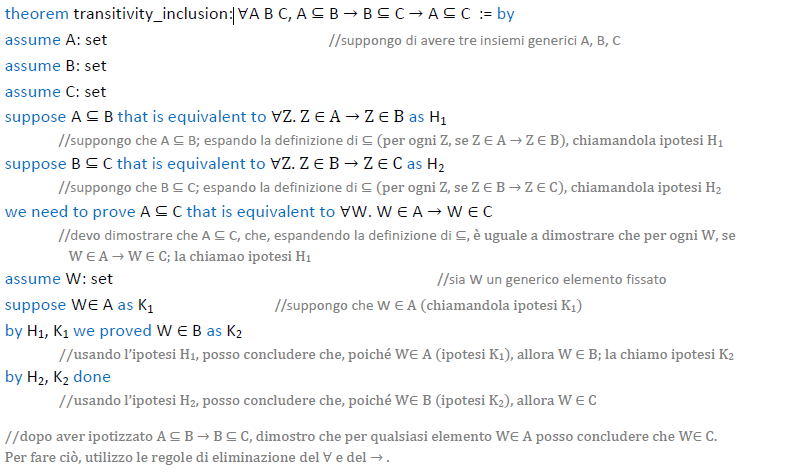
\includegraphics[height=.50\textheight,keepaspectratio]{lezione_1.50/lean_sample_code.PNG} % essenzialmente resiza l'immagine
    \begin{center}
        \caption{\label{fig:lean_sample_code}Dimostrazione teorema di riflessività dell'inclusione.} % label fuori da caption spesso non va, mettilo dentro
    \end{center}
\end{figure}
\end{document}